\chapter{Methodology}

We conducted experiments to gain insights into the proposed methods for researching the appliance of nD-Laplace for clustering algorithms.
The experiment results are used to evaluate our method against other literature.
In this chapter, we explain:
\begin{enumerate}
      \item Research design: The background and research questions are explained.
            Furthermore, we explain the datasets and privacy mechanisms used in the experiments.
      \item Data collection: The methods used to collect the data necessary to answer the research questions.
            These are methods for running experiments to collect data about utility and privacy.
      \item Data analysis: We explain how we analyze the data collected in the previous step.
\end{enumerate}

\section{Research design}
This section describes the overall setup of the research.
\subsection{Research background}
Clustering data is a crucial part of machine learning, aiming to discover patterns in the data that may not be immediately visible to the human eye.
To achieve this, the data is trained on large datasets.
However, storing such data is unsafe, as unauthorized access could lead to breaches.

\gls{ldp} has been introduced to safeguard user privacy while preserving data patterns.
Adding local noise means the plain data is never stored on a central server.
But, the limited available data in the local view distorts the patterns excessively in each noise addition.

Current literature has attempted to address this challenge, but the solutions fall short.
They either require modifications to the clustering algorithm or lack practical applicability due to the use of synthetic data.
Existing literature focuses mainly on 2-dimensional data with K-Means as the clustering algorithm.

To address these limitations, we propose a new \gls{ldp} method called nD-Laplace, utilizing distance to preserve data patterns using the concept of \gls{gi}. \newline
Our method enables secure training of clustering algorithms based on input-perturbation.
Due to this approach, we can train multiple clustering algorithms without modifications and extend them to n-dimensional data.
We will test three variants of the nD-Laplace mechanism to assess their utility and privacy characteristics.
\begin{enumerate}
      \item nD-Laplace: Plain mechanism without any additions for truncation.
      \item grid-nD-Laplace: Mechanism with truncation using grid-remapping (See Equation: \ref{alg:grid-remapping-laplace}).
      \item density-nD-Laplace: Mechanism with truncation using density-remapping (See Equation: \ref{alg:optimal-remapping-laplace}).
\end{enumerate}
We will compare the kD-Laplace mechanism to Piecewise, which is another \gls{ldp} mechanism (See Section \ref{theory:literature-review}) and assess the effectiveness of the proposed kd-Laplace variants.

This research combines real-world and synthetic data to demonstrate practical applicability.
Extensive external and internal validation experiments will be conducted to establish the method's practical relevance and effectiveness.


\subsection{Research questions}
The main question of the research is as follows: \newline \newline
\textit{"How can the nD-Laplace mechanism be applied in training privacy-preserving clustering algorithms on distributed n-dimensional data?"} \newline
This question is divided into four smaller sub-questions:
\begin{enumerate}
      \item \textit{RQ1: How can the 2D-Laplace, 3D-Laplace, and nD-Laplace approaches be adapted to train privacy-preserving clustering algorithms?} \newline
            This research question investigates the applicability of the different variants of the nD-Laplace mechanism for training clustering algorithms.
      \item \textit{RQ2: How can the noise generated by nD-Laplace outside the data boundary be remapped to inside the data domain?} \newline
            This research question extends grid-remapping (See Equation: \ref{alg:grid-remapping-laplace}) and density-remapping (See Equation: \ref{alg:optimal-remapping-laplace}) to be used with nD-Laplace for clustering.
      \item \textit{RQ3: How can one optimize the computational complexity when implementing grid and density-remapping using the nD-Laplace mechanism?} \newline
            This research question investigates the computational complexity of the grid-remapping and density-remapping algorithms.
      \item \textit{RQ4: How do dataset characteristics impact the nD-Laplace mechanism for utility and privacy?} \newline
            In this research question, we evaluate the dataset characteristics and their influence on nD-Laplace.
            Also, we investigate if we can improve the utility and privacy of kd-Laplace by adopting grid-nD-Laplace and density-nD-Laplace (\ref{fig:optimal-remapping}).
            We use several hypotheses questions to answer research question 3.

            In the last two hypotheses, we specifically focus on the K-Means clustering algorithm to test our hypotheses.
            The choice of K-Means is due to its simplicity, making it suitable for our hypothesis tests.
            Also, we assume that the K-Means results are representative of the other clustering algorithms.
            \begin{enumerate}
                  \item \textit{H1: Adding remapping based on density improves utility without sacrificing privacy:}
                        Since the noise is updated based on the density of the data points, the clusters stay preserved (\ref{alg:optimal-remapping-laplace}).
                        As a result, the utility increases while the data points remain indistinguishable.
                        Therefore, we have extended our mechanism with density remapping and named it density-kD-Laplace.
                  \item \textit{H2: The privacy leakage (adversary advantage) and utility increases for more dimensions:}
                        The hypothesis arose from our observation while investigating/implementing kD-laplace(\ref{theory:privacy-utility-nd}).
                        Adding more dimensions (5 >) decreases the added noise gradually, increasing utility.
                        On the other hand, privacy is expected to decrease because the noise is less.
                  \item \textit{H3: The shape of the data negatively impacts the kd-Laplace mechanism in terms of privacy and utility:}
                        Because the mechanism heavily relies on Euclidean distance, the shape (distance between the data points) can ultimately harm utility and privacy.
                        We have already observed this difference when comparing the heart and seed datasets in research questions 1 and 2.
                        But, to rule out the potential impact of the number of data points (the heart dataset has 2126 samples and the seed-dataset 210), we generate three synthetic datasets, each with 1000 samples (See section \ref{datasets-section}).
            \end{enumerate}
\end{enumerate}

\subsection{Datasets} \label{datasets-section}
For this research, we selected two real-world datasets based on the related papers (\ref{theory:literature-review}).
The datasets are sourced from the UCI Machine Learning Repository \citep{noauthor_uci_nodate}.
\begin{enumerate}
      \item \textbf{Seeds dataset} \footnote{http://archive.ics.uci.edu/ml/datasets/seeds}: This dataset was used in several related works and contains 210 samples with 7 (numerical) attributes.
            The dataset contains information about seeds, like kernel width and density.
            We conducted experiments with 2, 3, and 7 dimensions and decided to use the following features (based on the correlation between the features):
            \begin{enumerate}
                  \item 2-dimensional data: area and perimeter.
                  \item 3-dimensional data: the kernel's area, perimeter, and length.
                  \item 7-dimensional data: All numerical features.
            \end{enumerate}
      \item \textbf{Heart dataset} \footnote{https://archive.ics.uci.edu/ml/datasets/cardiotocography}: This dataset is selected because of the mixed data and amount of instances.
            It has 23 attributes, including ten numerical attributes and 2126 samples.
            The dataset contains information about measurements of fetal heart rate (FHR) and uterine contraction (UC).
            We conducted experiments with 2, 3, and 10 dimensions and decided to use the following features (based on the correlation between the features):
            \begin{enumerate}
                  \item 2-dimensional data: FHR baseline and histogram-min.
                  \item 3-dimensional data: FHR baseline, histogram-min, and accelerations.
                  \item 10-dimensional data: All numerical features.
            \end{enumerate}
\end{enumerate}
The following datasets are for the H3 (shape) hypothesis investigated in research question 3.
For this purpose, we generated a 2-dimensional and 3-dimensional dataset with 1000 samples.
\begin{figure}[H]
      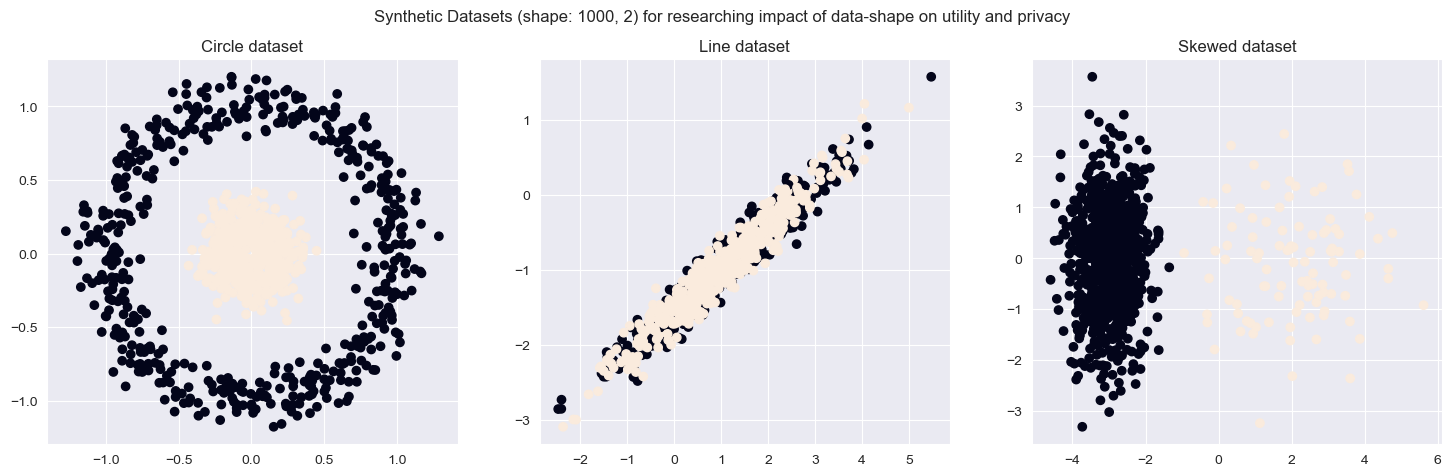
\includegraphics[width=1.0\textwidth]{Method//images/2d-shapes.png}
      \caption{Synthetic datasets with 1000 samples and 2-dimensions}
      \label{rq3:synthetic-datasets}
\end{figure}
\begin{figure}[H]
      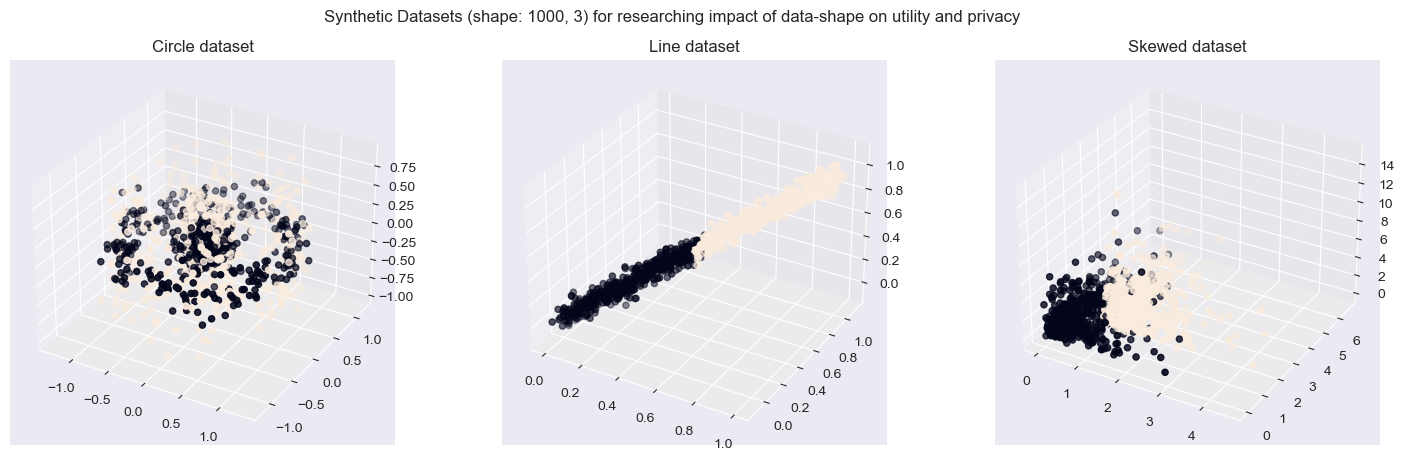
\includegraphics[width=1.0\textwidth]{3d-shapes.png}
      \label{rq3:synthetic-datasets-3d}
\end{figure}

\begin{enumerate}
      \item \textbf{Circle dataset:} Dataset with a circle shape.
      \item \textbf{Line dataset:} Dataset is a line (shape is much like the seeds dataset).
      \item \textbf{Skewed dataset:} Dataset samples are skewed/concentrated to one side (shape is much like the heart dataset).
\end{enumerate}

\subsection{Experiment setup}
We evaluate all privacy mechanisms by comparing them in utility and privacy.
To reduce the measurement bias of results, we executed them ten times for multiple privacy budgets and reported the average for each \citep{9679364}.
\begin{enumerate}
      \item The experiments run ten times, and we report the mean.
      \item All experiments run for multiple epsilons: ${0.5, 0.7, 1, 1.5, 2, 3.5, 5, 7, 9}$.
\end{enumerate}
\newpage

\subsection{Environmental setup}
For running the experiments, we use 16GB RAM and an i7-10750H 2.6Ghz processor.
The experiments are run using a Docker container which runs a pre-configured distribution of Linux Alpine.
It includes a pre-installed Anaconda environment for Python \footnote{https://github.com/devcontainers/images/tree/main/src/anaconda}\footnote{tag: mcr.microsoft.com/devcontainers/anaconda:0-3}.
We run the container using the dev-container feature for visual-studio code \footnote{https://code.visualstudio.com/docs/devcontainers/containers}.
This allows us to create a reproducible experiment environment.
\subsubsection{Libraries \& code versions}
We use Python version 3.9.13 with Jupyter Notebook for creating a reproducible experimental environment.
The packages for Python are:
\begin{itemize}
      \item Scikit-learn: 1.0.*
      \item Yellow-brick: 1.5
      \item Numpy: 1.24.*
      \item Pandas: 2.0.*
      \item Seaborn: 0.11.*
      \item Mathplotlib: 3.5.*
\end{itemize}

\section{Data collection}
This section explains what methods/ algorithms we use to collect the data necessary to answer the research questions.
\subsection{Hyperparameter selection}
For the three different algorithms: K-Means, \gls{ap}, and OPTICS, we analyzed the most important decisions regarding hyperparameter selection (See section \ref{paragraph:choosing-r}).
This section gives a short list and explanation of the parameters we used throughout the experiments.
\subsubsection{K-Means}
\begin{table}[H]
      \begin{tabular}{|l|p{6cm}|l|l|}
            \hline
            Parameter & Description                          & Value                                                         & Dataset        \\ \hline
            K-value   & \makecell{Calculated based \\ on the silhouette method} & k=2 & \makecell{Heart dataset (2 \& 9 dimensions) \\ Seeds dataset (2 \& 7 dimensions) \\ Line dataset (2 \& 3 dimensions}  \\ \hline
            K-value   & ""                                   & k=4  & \makecell{Heart dataset (3 dimensions) \\ Skewed dataset (3 dimensions)}   \\ \hline
            K-value   & ""                                   & k=5 & \makecell{Seeds dataset (3 dimensions) \\ Skewed dataset (2 dimensions)} \\ \hline
            K-value  & ""                                    & k=7 & \makecell{Circle dataset (2 dimensions)} \\ \hline
            K-value  & ""                                    & k=9 & \makecell{Circle dataset (3 dimensions)} \\
            \hline

      \end{tabular}
      \caption{K-Means hyperparameters for datasets}
      \label{tab:kmeans-formula-dataset-2}
\end{table}
The above table shows the relevant hyperparameters for the K-Means clustering algorithm.
The hyperparameter differs for each dataset, so we must display it for each.
This hyperparameter is the k-value used to determine the number of clusters.
The "value" column shows the value we used for the experiments, with the corresponding "elbow" plot in the referenced figure.
\subsubsection{Agglomerative clustering}
\begin{table}[H]
      \begin{tabular}{|l|p{6cm}|l|l|l|}
            \hline
            Parameter & Description & Value & Dataset(s) \\
            \hline
            \makecell{Number of                          \\ clusters} & This is decided based on silhouette method with the SC metric \ref{theory:clustering-agglomerative} & n\_clusters=2 & \makecell{Heart-dataset (2 dimensions) \\ Seeds dataset (2 \& 3 dimensions) \\ Line dataset (2 dimensions)} \\ 
            \hline
            \makecell{Number of                          \\ clusters} & ""          & n\_clusters=3 & \makecell{Heart-dataset (9 dimensions) \\ Line dataset (3 dimensions)}          \\
            \hline
            \makecell{Number of                          \\ clusters} & ""          & n\_clusters=4 & \makecell{Seeds-dataset (7 dimensions) \\ Heart dataset (3 dimensions) } \\
            \hline
            \makecell{Number of                          \\ clusters} & ""          & n\_clusters=6 & \makecell{Skewed dataset (2 dimensions)}  \\
            \hline
            \makecell{Number of                          \\ clusters} & ""          & n\_clusters=7 & \makecell{Circle dataset (2 dimensions)} \\
            \hline
            \makecell{Number of                          \\ clusters} & ""          & n\_clusters=9 & \makecell{Circle dataset (3 dimensions) \\ Skewed dataset (3-dimensions)} \\
            \hline

      \end{tabular}
      \caption{Agglomerative clustering hyperparameters for the datasets}
      \label{tab:ap-formula-sklearn}
\end{table}
The above table shows the relevant hyperparameters for the \gls{ag} clustering algorithm per dataset.
Because the hyperparameters "n\_clusters" rely heavily on the number of dimensions, each dataset's dimensions were provided.
For the "n\_clusters," we used the \gls{sc} in corporation with the elbow method to determine the number of clusters.
In addition, there is the "linkage," which is "ward" for all configurations (See Section \ref{theory:clustering-agglomerative}).
\newpage
\subsubsection{OPTICS}

\begin{table}[h]
      \begin{tabular}{|l|p{6cm}|l|l|}
            \hline
            Parameter      & Description                                                                                                    & Value       & Dataset                    \\
            \hline
            Minimum points & Decided using the formula $minPts = n * 2$, where n is the number of features (\ref{theory:clustering-dbscan}) & $minPts=4$  & \makecell[l]{Seeds dataset \\ Heart dataset \\ Circle dataset \\ Line dataset \\ Skewed dataset \\ (2-dimensions)}  \\
            \hline
            Minimum points & ""                                                                                                             & $minPts=6$  & \makecell[l]{Seeds dataset \\ Heart dataset \\ Circle dataset \\ Line dataset \\ Skewed dataset \\ (3-dimensions)} \\
            \hline
            Minimum points & ""                                                                                                             & $minPts=14$ & \makecell[l]{Seeds dataset \\ (7-dimensions)}  \\
            \hline
            Minimum points & ""                                                                                                             & $minPts=18$ & \makecell[l]{Heart dataset \\ (10-dimensions)} \\
            \hline
      \end{tabular}
      \caption{OPTICS  hyperparameters for datasets}
      \label{tab:dbscan-formula-sklearn}
\end{table}
The above table shows the relevant hyperparameters for the \gls{optics} clustering algorithm for each dataset.
Because the minimum points depend on the number of dimensions, we must display them for each dataset (See Section: \ref{theory:clustering-dbscan}).
We omitted the synthetic datasets for the same reason specified for \gls{ap}.
The first two rows display the minimum points for the datasets that have 2 and 3-dimensional data.
The last two rows display the minimum points for the datasets that have 7 and 10-dimensional data.
\newpage
\subsection{Utility and privacy evaluation}
\subsubsection*{Utility}
To measure cluster utility, both internal and external validation methods are used:
%Based on section \ref{theory:evaluate}, we can conclude that the corresponding literature mainly evaluates one clustering algorithm and not multiple ones.
%Furthermore, it can be concluded that if we only want to measure the coherence of the clusters, we can use an internal validation method. If we want a concrete measurement compared to the non-private version, an external validation method can be used.
%Both measurements are important to evaluate, so we use both external and internal validation. \newline
\mycomment{
      The Scikit-learn package provides the implementation for these metrics.
      With the underlying formulas:
      \begin{equation}
            AMI(U, V) = \frac{MI(U, V) - E(MI(U, V))}{avg(H(U), H(V)) - E(MI(U, V))}
      \end{equation}
      \capequation{Adjusted Mutual Information formula \citep{vinh_information_nodate-2,hubert_comparing_1985-1}}
      \begin{gather}
            RI = \frac{a + b}{C^{n}_{2}} \\
            ARI = \frac{RI - E(RI)}{max(RI) - E(RI)}
      \end{gather}
      \capequation{(Adjusted) Rand Index formula \citep{rand_objective_1971, hubert_comparing_1985-1}}
}
\begin{enumerate}
      \item \textbf{External validation: }
            The external validation is measured by comparing the labels of non-private trained clustering algorithms with those trained using a privacy mechanism.
            The outcome is between 0 and 1, where 1 indicates the highest similarity (thus the best result).
            AMI (Adjusted Mutual Information) is used to assess the external validity of the clustering algorithms (See Section \ref{theory:evaluate}).
      \item \textbf{Internal validation: }
            The internal validation measures the intrinsic properties of the clustering algorithms.
            The outcome is a value between -1 and 1 for the SC evaluation.
            Where -1 indicates incorrect and 1 dense clustering (See Section \ref{theory:evaluate}).
\end{enumerate}
Because the clustering algorithms rely on Euclidean distance, we need to apply some data standardization.
For this purpose, we use standard scaling provided by the Scikit-learn package \footnote{https://scikit-learn.org/stable/modules/preprocessing.html}.

\subsubsection{Privacy}
Privacy is hard to quantify, but we can measure the privacy loss/gain by calculating the Euclidean distance between the non-perturbed and perturbed data.
In addition, we evaluate privacy by simulating a membership inference attack and calculating the adversary advantage.
\begin{enumerate}
      \item \textbf{Privacy distance: }
            The first measurement we evaluate is the distance between the dataset's non-private and private variants.
            This metric gives us a sense of how much extra distance (and privacy) the privacy mechanisms offer compared to the non-private variant.
            %We call this "disclosure risk" because it measures how much noise is added.
            To this end, the average Euclidean distance is measured and reported per epsilon. A higher distance indicates more privacy.
      \item \textbf{Adversarial advantage: }
            We use the Membership Inference Attack (MIA) that Shokri et al. proposed with the implementation that was provided by Adversarial Robustness Toolkit (ART) \citep{nicolae_adversarial_2019}.
            An earlier study also explored this attack to evaluate differential privacy.
            Similar to this attack, we train a classifier with perturbed data and evaluate it using non-perturbed data (test-data / shadow-data) \citep{zhao_not_2020}.
            We consider a semi-supervised setup (Figure \ref{figure:MIA-semi-supervised}), where we train a classifier with the perturbed data and evaluate it using non-perturbed data (test-data / shadow-data).
            For the classifier, we use a RandomForestClassifier \citep{rigaki_survey_2021}.
            Finally, we evaluate the adversary advantage (percentage) using $TPR - FPR$ \citep{yeom_privacy_2018}.
            Figure: \ref{figure:mi-attack} provides a visual setup of the experiment.

            Although the adversary advantage is a proven method for measuring MI attacks, we also include the TPR as an essential measurement.
            This metric is most interesting to us because this displays the percentage of the actual leaked labels (see Section \ref{theory:attack-evaluation}).
            \begin{figure}[H]
                  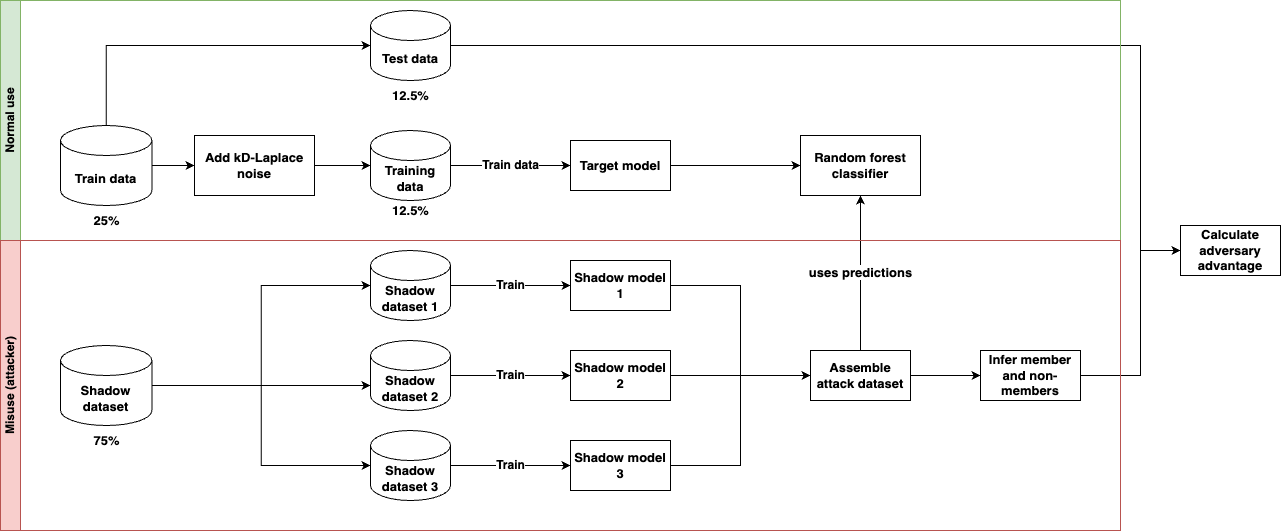
\includegraphics[width=1.1\textwidth]{Method/images/MI-setup.png}
                  \caption{Member inference attack using shadow models. The green swim lane illustrates the normal setup, and the red swim lane projects the adversary steps.}
                  \label{figure:mi-attack}
            \end{figure}
            The figure above visually represents the \gls{mia} attack we set up using semi-supervised learning.
            \begin{enumerate}
                  \item The green swim line presents the setup for legitimate system usage.
                        Here, we use a general setup for a supervised machine learning setup.
                        First, the data is split into test/train data, where only the training data is private.
                  \item Then, the K-Means clustering algorithm is privately trained, and the labels are used with the RandomForestClassifier.
                  \item The red swim line presents the adversary's steps.
                        This approach uses Shokri et al. attack setup using shadow models \citep{shokri_membership_2017}.
                        The random shadow datasets and classifiers are combined into an attack dataset.
                  \item Then, the attacker tries to infer the training data from the attack dataset using the classifier's predictions.
                  \item Finally, we calculate the adversary advantage using the inferred labels and the original labels.
            \end{enumerate}
            The attacker could infer many original labels if the adversary advantage or \gls{tpr} is high.
            In this case, a lower score is better than a lower score.
\end{enumerate}
%\begin{algorithm}[H]
  \caption{Black-box inference attack}\label{alg:shokri-mi}
  \begin{algorithmic}
    \Ensure $z$
    \State $x_{target}, y_{target}, x_{shadow}, y_{shadow} = split(X)$ \Comment 75\% shadow data
    \State $x_{target-train}, y_{target-train} = split(xy_{target})$ \Comment 12.5\% train data
    \State $x_{target-test}, y_target_test = split(xy_{target})$ \Comment 12.5\% test data
    \State $Z = 2/3nD-Laplace(x_{target-train})$ 
    \State $private_classifier = RandomForestClassifier(Z, y_{target-train})$ \Comment See scikit-learn (\textbf{Bron})
    \For{three times}
      \State $dataset_{shadow} = generate_shadow_datasets$ \Comment using ART implementation
    \EndFor

  \end{algorithmic}
\end{algorithm}
\subsection{Research roadmap} \label{research-roadmap}
This section explains the experiments' setup and the result reporting order.
\begin{enumerate}
      \item Cluster utility: The mechanisms kD-Laplace and Piecewise are compared using the external and internal validation methods.
            We report the \gls{ami} and SC in the results for both mechanisms and each dataset.
            For this experiment, we only consider real-world datasets.
      \item Mechanism utility: Both mechanisms are compared against each other by evaluating the \gls{ami} and \gls{sc}.
            In this research, we also conduct experiments to assess the impact of the number of dimensions on the utility of each dataset.
      \item Mechanism privacy: We do the same for utility, but now with privacy.
            For this purpose, we evaluate the adversary advantage and privacy distance.
      \item Mechanism comparison: Now we established the performance of nD-Laplace and Piecewise, we compare the different variants of kD-Laplace.

\end{enumerate}
%Therefore, we analyze our method according to a popular attack: Membership inference attack.
%For this purpose, we make use of a black-box Member inference attack, called "HopSkipJump" \citep{chen_hopskipjumpattack_2020,li_membership_2021}.
%This attack is evaluated using a semi-supervised setup, as proposed in this figure: \ref{fig:unsupervised-mia-attack}.
%We will make use of a decision tree model for classification but can be replaced by any other classification model.
%Both the private and non-private trained models are evaluated based on the true positive rate (TPR) and false positive rate (FPR).
%Respectively meaning, the TPR is higher if the MIA is successful and likewise the FPR if the MIA is unsuccessful.
%We hypothesize that the private model leverages a higher FPR in comparison to the non-private variant.
%Therefore, it is more convenient to apply the geo-indistinguishability as an error metric provided in \ref{eq:geo-as-an-error}.
\mycomment{
      We propose several solutions for open issues based on the theoretical framework. \newline
      \subsubsection{Choosing r: } Based on the idea of Chatzikokolakis et al. to lower the radius size if the place is crowded, we can do the same with clustering.
      For this, we could use a metric like the standard division.
      This metric does precisely this by providing the deviation from the mean:

      This metric increases based on the clutteredness of the data, which allows us to generate a radius $r$ automatically regardless of domain.
      Therefore, we depend on the reconfigurability of epsilon entirely on privacy level $l$.
      The generic standard deviation can be defined as:
      \begin{equation}
            \sigma = \sqrt{\frac{\sum{(x_i - \mu)^2}}{n}}
      \end{equation}
      The $\sigma$ being our diameter $d$, the radius $r$ is then calculated as $\frac{d}{2}$. \newline
}
\mycomment{\subsubsection{Truncation:}
      We explained the theory for truncation earlier in paragraph \ref{theory:truncation}.
      The methods proposed work correctly for a geographic map where other (historical) locations for remapping are available.

      However, it is difficult to apply this to data clustering.
      The number of data points is unknown beforehand, so we may remap to a location that is too far away.
      This way, we lose essential distance information, which hurts the clustering.
      Also, the truncation threshold is so clear (the points are outside the known 2D domain) that we do not have to rely on historical data for remapping.
      Our algorithm can be much more straightforward by re-calculating the noise until it is within the domain:
}
\mycomment{
      \begin{equation}
            T(x_{max}, x_{min}, z, x_0) \begin{cases} z &\text{if } 0 < 1 \\ T(x_{max}, x_{min}, planarLaplace(epsilon, x_0), x_0)  &\text{else} \end{cases}
      \end{equation}
}
%\begin{algorithm}
  \caption{Truncation algorithm ($T(\min, \max, x_0, z)$) for clustering with planar Laplace}\label{alg:truncaction-rq1}
  \begin{algorithmic}
    \Ensure $z$
    \State $x_1, y_1 \gets x_{min}$
    \State $x_2, y_2 \gets x_{max}$
    \State $z_x, z_y \gets z$
    \If{$x_1 < z_x < x_2$ and $y_1 < z_y < y_2$}
    \State \Return $z$
    \Else
    \State $x, y \gets x_0$
    \State $z_2 \gets LP(\epsilon, x, y)$ \Comment See formula 3.3.
    \State \Return $T(x_{min}, x_{max}, x_0, z_2)$ \Comment Rerun recursively
    \EndIf
  \end{algorithmic}
\end{algorithm}
%This algorithm uses $x_{min}$ and $x_{max}$ to re-calculate the points within the domain using respectively the minimum X/Y and maximum X/Y.
%An example of this is visualized:
%\begin{figure}[h]
%  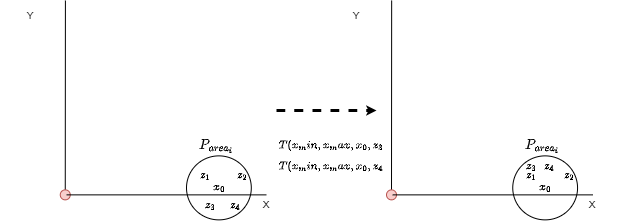
\includegraphics[width=0.8\textwidth]{Method/images/truncation-rq1.png}
%  \label{fig:truncation}
%  \centering
%  \caption{Representation of the remapping algorithm for clustering for points $z_3$ and $z_4$ }
%\end{figure}

%\subsubsection{Probability metric $K(x)(Z)$}
%\todo[inline]{Explain the probability metric $K$ we used}

%\newpage
%\subsubsection{Algorithm}
%The full algorithm for the perturbation:
%\begin{algorithm}[H]
  \caption{Full algorithm for perturbing cluster data based on planar/2D-Laplace \citep{DBLP:journals/corr/abs-1212-1984}}\label{alg:rq1}
  \begin{algorithmic}
    \Require $x \in X$  \Comment 2D array of points
    \Require $l \in R^ +$
    \Ensure $z \in Z$ \Comment 2D array of perturbed points
    \State $r = \frac{\sigma}{2}$ \Comment formula 4.1
    \State $\epsilon = \frac{l}{r}$ \Comment Calculating privacy budget \citep{DBLP:journals/corr/abs-1212-1984}
    \State $x_{min} \gets min(X)$
    \State $x_{max} \gets max(X)$
    \State $Z \gets []$
    \For{$point_i \in X$}
    \State $\theta \gets [0, \pi2]$       \Comment Random noise for $\theta$
    \State $p \gets [0, 1]$
    \State $z_i \gets C{_\epsilon}{^{-1}}(p)$       \Comment formula 3.2
    \State $z_i \gets T(x_{min}, x_{max}, point_i, z_i)$ \Comment algorithm 1.
    \State $x_{perturbed} \gets point_{i_x} + (z_{i_x} * \cos(\theta)) $ \Comment add noise to x-coordinate
    \State $y_{perturbed} \gets point_{i_y} + (z_{i_y} * \sin(\theta)) $ \Comment add noise to y-coordinate
    \State append $x_{perturbed}, y_{perturbed}$ to Z
    \EndFor
    \State \Return Z
  \end{algorithmic}
\end{algorithm}
%% We apply the theory for planar laplace proposed by \citep{DBLP:journals/corr/abs-1212-1984}

\section{Data analysis}
For the data analysis, we utilize visualization libraries in Python, primarily Matplotlib, in combination with Seaborn.
\begin{itemize}
      \item Line/bar plot: These plots visualize comparisons between the different privacy mechanisms.
            The different epsilon values are displayed on the x-axis, and the utility/privacy metric is displayed on the y-axis.
      \item Heatmap plot: These plots visualize the interaction between dimensions and epsilons.
            This way, we can display two categorical values (dimension/epsilon) and one continuous value.
\end{itemize}
%\todo[inline]{Added ideas for research question 3}

%In addition to testing the hypotheses, we also want to investigate the behavior of our mechanism in more detail.
%\begin{enumerate}
%\item Research the applicability of the mechanism for other clustering algorithms, like hierarchical clustering.
%  \item Research the impact of the data shape on privacy leakage.
%\item Explore options to extend the method to support categorical data.
%\item Explore options to extend the method to support binary data.
%\item Research possibility to include the privacy mass: \ref{equation:privacy-mass-a}.
%\end{enumerate}
